\documentclass[12pt]{article}
\usepackage{amsthm,amssymb,amsmath,amsfonts}
\usepackage[a4paper, top=25mm, bottom=30mm, left=25mm, right=25mm]{geometry}
\usepackage[pagebackref=false,colorlinks,linkcolor=black,citecolor=black]{hyperref}
\usepackage[nameinlink]{cleveref}
 \AtBeginDocument{%
    \crefname{equation}{برابری}{equations}%
    \crefname{chapter}{فصل}{chapters}%
    \crefname{section}{بخش}{sections}%
    \crefname{appendix}{پیوست}{appendices}%
    \crefname{enumi}{مورد}{items}%
    \crefname{footnote}{زیرنویس}{footnotes}%
    \crefname{figure}{شکل}{figures}%
    \crefname{table}{جدول}{tables}%
    \crefname{theorem}{قضیه}{theorems}%
    \crefname{lemma}{لم}{lemmas}%
    \crefname{corollary}{نتیجه}{corollaries}%
    \crefname{proposition}{گزاره}{propositions}%
    \crefname{definition}{تعریف}{definitions}%
    \crefname{result}{نتیجه}{results}%
    \crefname{example}{مثال}{examples}%
    \crefname{remark}{نکته}{remarks}%
    \crefname{note}{یادداشت}{notes}%
    \crefname{observation}{مشاهده}{observations}%
    \crefname{algorithm}{الگوریتم}{algorithms}%
    \crefname{cproof}{برهان}{cproofs}%
}

\usepackage{tikz}
\usepackage{graphicx}
\usepackage{color}

\usepackage{setspace}
\doublespacing

\usepackage{titletoc}
\usepackage{tocloft}
\usepackage{enumitem}

\usepackage{algorithm}
% \usepackage[noend]{algpseudocode}
\usepackage[noend]{algorithmic}
\renewcommand{\algorithmicrequire}{\textbf{Input:}}
\renewcommand{\algorithmicensure}{\textbf{Output:}}

\usepackage{tabularx}
\makeatletter
\newcommand{\multiline}[1]{%
  \begin{tabularx}{\dimexpr\linewidth-\ALG@thistlm}[t]{@{}X@{}}
    #1
  \end{tabularx}
}
\makeatother

\usepackage{float}
\usepackage{verbatim}
\makeindex
\usepackage{sectsty}
\usepackage{xepersian}
\SepMark{-}
\settextfont[Scale=1.2,Path=fonts/,BoldFont=B Nazanin Bold.ttf]{B Nazanin.ttf}
\setlatintextfont{Times New Roman}
\renewcommand{\labelitemi}{$\bullet$}

\theoremstyle{definition}
\newtheorem{definition}{تعریف}[section]
\newtheorem{remark}[definition]{نکته}
\newtheorem{note}[definition]{یادداشت}
\newtheorem{example}[definition]{نمونه}
\newtheorem{question}[definition]{سوال}
\newtheorem{remember}[definition]{یاداوری}
\newtheorem{observation}[definition]{مشاهده}
\theoremstyle{theorem}
\newtheorem{theorem}[definition]{قضیه}
\newtheorem{lemma}[definition]{لم}
\newtheorem{proposition}[definition]{گزاره}
\newtheorem{corollary}[definition]{نتیجه}
\newtheorem*{cproof}{برهان}



\begin{document}
\fontsize{12pt}{14pt}\selectfont

\begin{minipage}{0.1\textwidth}

\end{minipage}%
\hfill%
\begin{minipage}{0.6\textwidth}\centering
\fontsize{10pt}{10pt}\selectfont
به نام خداوند \\
تئوری یادگیری ماشین \\
دکتر سیدصالحی\\
جلسه سوم
 \\
\vspace{0.25cm}
\begingroup
\fontsize{8pt}{8pt}\selectfont
دانشکده ریاضی و علوم کامپیوتر \\
اسفند ماه 1402\\
\endgroup
\end{minipage}%
\hfill%
\begin{minipage}{0.1\textwidth}
\end{minipage}

\vspace{0.5cm}

\noindent\rule{\textwidth}{1pt}

% \begin{abstract}
% \noindent
% مقدمات نگرش احتمالاتی به مسئله 
% \lr{learning}
% و آشنایی با دو تخمین‌گر 
% \lr{Maximum-Likelihood (ML)}
% و
% \lr{Maximum A Posteriori (MAP)}
% و سپس بررسی این دیدگاه در رابطه با مسئله 
% \lr{Regression}
% \end{abstract}


\section*{$Probabilistic\:Perspective\:of\:
Learning$}
\subsubsection*{$Probabilistic\:Unsupervised\:Learning$}
یکی از دسته مسائل یادگیری که پیش تر با آن آشنا شده اید مسائل
\lr{unsupervised}
هستند. برای این دسته از مسائل نیز میتوان یک دیدگاه احتمالاتی داشت. برای مثال اگر با دیدگاه احتمالاتی به مسئله خوشه بندی نگاه کنید میتوان فرض کرد که هر کدام از خوشه های ما از توزیع های احتمالاتی پیروی میکنند و با استفاده از داده ها به توزیع مدنظر رسید آنگاه هر دیتای جدیدی را میتوان با استفاده از توزیع هایی که بدست آورده ایم به یکی از خوشه‌ها تخصیص داد.

\begin{figure}[h]
    \centering
    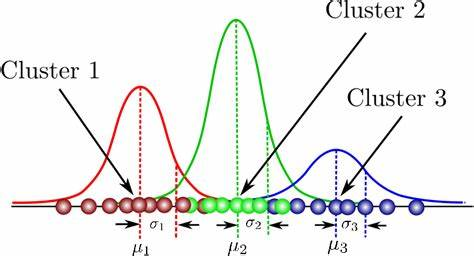
\includegraphics[width= 0.8\textwidth]{figs/GaussianMixtureModel.jpeg}
    \caption{فرض قرار دادن یک توضیع $gaussian$ در دیتا}
    \label{fig:gaussian_mixture_model}
\end{figure}

\subsubsection*{$Generative\:Approach$}
دیدگاهی است که در آن فرض میکنیم که در ساختار داده‌ها توزیع 
\lr{p}
را داریم و بدنبال یادگرفتن توزیع 
\lr{p}
میرویم تا بتوانیم کارهایی از قبیل تولید داده انجام دهیم. 
\href{http://cs231n.stanford.edu/slides/2017/cs231n_2017_lecture13.pdf}{\lr{more information}}


\subsection*{رویکردهای اصلی $density\:estimation$}
دو دسته رویکرد برای این نوع تخمین وجود دارد.
\begin{itemize}
    \item \lr{parametric}:
    موردی که فعلا مورد بحث در کورس است و با تخمین پارامترهای توزیع سرکار دارد.
    \item \lr{non-parametric} هیچ مدل پارامتری خاصی در نظر گرفته نمی شود.
\end{itemize}
در 
\lr{parametric}
ها نیز دو نوع دیدگاه برای تخمین 
$\theta$
وجود دارد بصورتی که دسته ای از افراد یک عدد ثابت را به عنوان پارامتر در نظر میگیرند و حال بدنبال تخمین آن عدد میروند
(\lr{MLE})
درصورتی که دسته دیگر آن را 
\lr{random variable}
در نظر میگیرند و بدنبال بدست آوردن تخمینی از توزیع آن هستند
(\lr{MAP, Bayesian Estimator}).
\\
\\
فرض کنید فضای یک بعدی زیر را همراه توضیعی داریم:
\begin{figure}[h]
    \centering
    \includegraphics[width=0.7\textwidth]{figs/ExNormDist.png}
    \label{fig:your_label}
\end{figure}

ما توضیع را نمیدانیم ولی یک خانواده را فرض و میخواهیم از میان آنها توضیعی از میان آن خانواده بخصوص که سمپل ها ازش $generate$ شدن را پیدا کنیم.
\\
\\
خانواده توضیع نرمال را در نظر میگیریم و پارامتر هاش رو تغییر میدیم:

\begin{figure}[h]
    \centering
    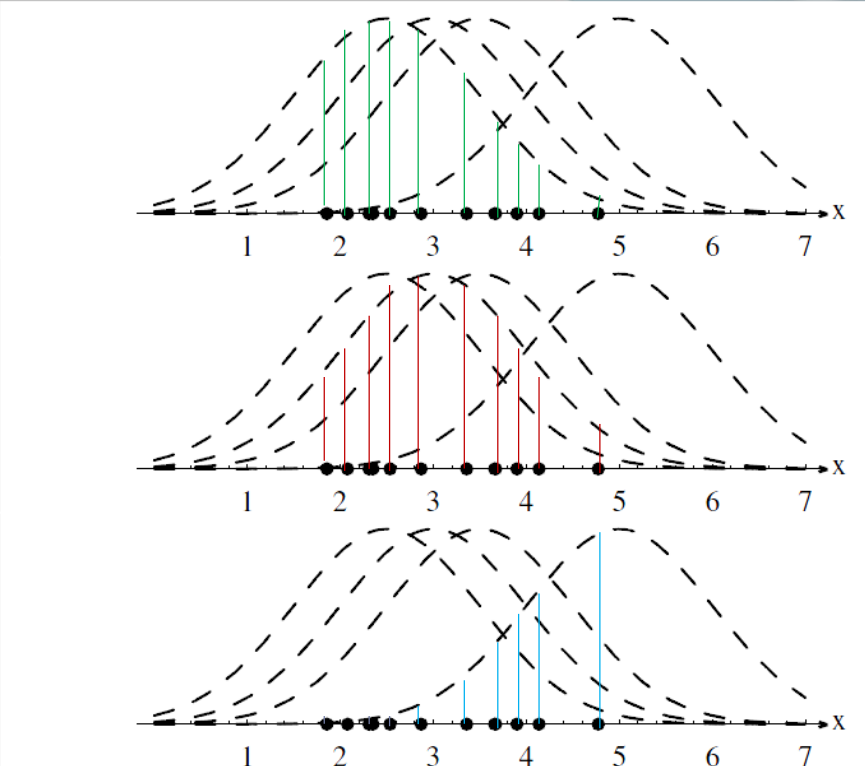
\includegraphics[width=0.8\textwidth]{figs/normalDistMLE.png}
    \label{fig:your_label}
\end{figure}

\begin{figure}[h]
    \centering
    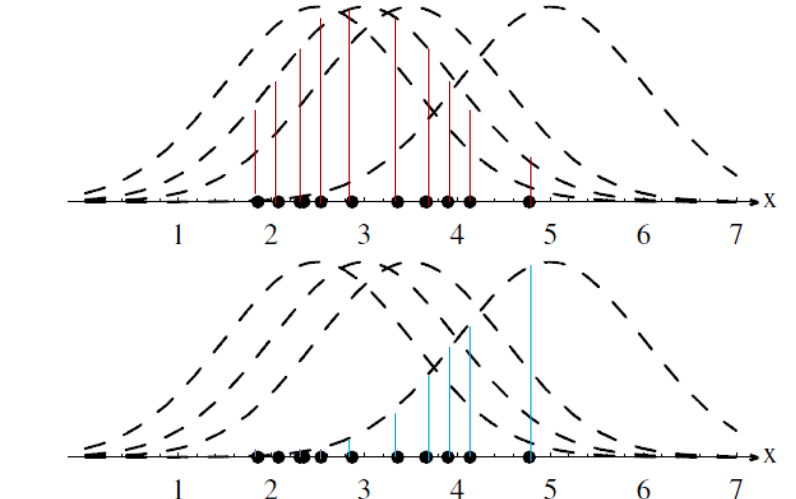
\includegraphics[width=0.8\textwidth]{figs/normalDistMLE2.png}
    \label{fig:your_label}
\end{figure}


\section*{$MLE$}
فرض کنید دسته ای از سمپل ها به شکل
$D = \{x^{(1)}, x^{(2)}, ..., x^{(n)}\}$
داریم. همچنین فرض کنید خانواده توزیع نرمال را داشته باشیم در شرایطی که واریانس اعضا ثابت باشد و تنها پارامتری که بین اعضا متفاوت است 
$\mu$
باشد.


حال بدنبال بهترین توزیع نرمالی هستیم که به این داده ها فیت شود. فرض دیگری که میکنیم 
\lr{i.i.d}
بودن مشاهدات است.
پس داریم.
\[p(D|\theta) = \prod_{i=1}^{N} p(x^{(i)}|\theta)\]
و در 
\lr{MLE}
بدنبال یافتن مقداری هستیم که این احتمال را بیشینه کند.
\[\hat{\theta}_{ML} = \underset{\theta}{argmax} \,p(D|\theta)\]
برای راحت تر کردن محاسبات هم میتوانیم از فرمت لگاریتمی استفاده کنیم و از انجایی که در اینجا بدنبال 
\lr{argmax}
گرفتنیم حاصل خود عبارت بالا با لگاریتمش تفاوتی نخواهد داشت.
\[L(\theta) = ln \,p(D|\theta) = ln \prod_{i = 1}^{N} p(x^{(i)}|\theta) = \Sigma_{i=1}^{N} ln \,p(x^{(i)}|\theta)\]
\[\hat{\theta}_{ML} = \underset{\theta}{argmax}\,L(\theta) = \underset{\theta}{argmax}\, \Sigma_{i=1}^{N} ln \,p(x^{(i)}|\theta)\]

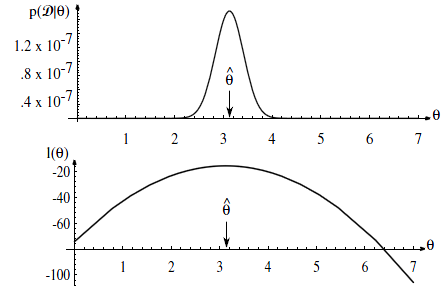
\includegraphics[width=\textwidth]{figs/Lograithm.png}

\subsection*{مثال $Bernoulli$ - گسسته}
در این مثال فرض کنید که آزمایش 
\lr{N}
بار پرتاب یک سکه را داریم بصورتی که 
\lr{m}
بار سکه شیر آمده است و بقیه دفعات را خط آمده است.
پس خانواده توزیع مسئله، توزیع برنولی است که به شکل زیر است.
\[p(x|\theta) = \theta^x (1 - \theta)^{1-x}\]
در این مسئله شیر آمدن را ۱ و خط آمدن را ۰ در نظر میگیریم و پارامتر 
$\theta$
را نیز معادل احتمال ۱ شدن یک بار پرتاب سکه میگیریم. 
بدین ترتیب برای آزمایشمان داریم.
\[p(D|\theta) = \prod_{i=1}^{N} p(x^{(i)}|\theta) = \prod_{i=1}^{N} \theta^{x^{(i)}} (1 - \theta)^{1 - x^{(i)}}\]
حال از تخمین‌گر استفاده میکنیم.
\[ln\,p(D|\theta) = \Sigma_{i=1}^{N}ln\,p(x^{(i)}|\theta)
    = \Sigma_{i=1}^{N} \{x^{(i)}\,ln\,\theta + (1 - x^{(i)})\,ln\,(1 - \theta)\}\]
حال باید مقدار اپتیمال را بدست آوریم.
\[\frac{\partial\, ln\,p(D|\theta)}{\partial\theta} = 0 \xrightarrow{}
    \theta_{ML} = \frac{\Sigma_{i=1}^{N} x^{(i)}}{N} = \frac{m}{N}\]

ولی این تخمین تخمین مناسبی نیست زیرا حالتی ممکن است پیش بیاد که سمپل ما مثال 3 از 3 بار رو آمده باشد و خب با تخمین 1 میشود که خب مناسب نیست. در اصطلاح به این حالت \lr{Overfitting} میگویند که بعدا با آشنا میشویم.

    
\subsection{مثال $Gaussian$ - پیوسته}
این بار بر روی خانواده توزیع نرمال با ثابت در نظر گرفتن پارامتر واریانس بدنبال تخمینی برای 
$\mu$
هستیم.
\[p(x|\mu) = \frac{1}{\sqrt{2\pi}\sigma}\exp^{-\frac{1}{2\sigma^2}(x - \mu)^2}\]
\[L(\mu) = ln\,p(x^{(i)}|\mu) = -ln\{\sqrt{2\pi}\sigma\} - \frac{1}{2\sigma^2}(x^{(i)} - \mu)^2\]
و حال برای بدست اوردن مقدار اپتیمال مشتق میگیریم.
\[\frac{\partial L(\mu)}{\partial \mu} = 0 \xrightarrow[]{} \frac{\partial}{\partial\mu}(\Sigma_{i=1}^{N} ln\,p(x^{(i)}|\mu)) = 0 \xrightarrow[]{}
    \Sigma_{i=1}^{N} \frac{1}{\sigma^2}(x^{(i)} - \mu) = 0\]
نتیجتا
\[\hat{\mu}_{ML} = \frac{1}{N}\Sigma_{i=1}^{N}x^{(i)}\]

\section*{\lr{MAP}}
در اینجا علاوه بر فرضیاتی که برای تخمین‌گر 
\lr{ML}
داشتیم فرض میکنیم که پارامتر یک متغیر تصادفی است. همچنین 
\lr{prior distribution}
آن را نیز داریم.
حال بدنبال این هستیم تا پارامتر را به نحوی بدست بیاوریم که توزیع 
\lr{posterior}
را بیشینه کنیم.
\[\hat{\theta}_{MAP} = \underset{\theta}{argmax}\, p(\theta | D)\]
طبق قانون بیز داریم.
\[p(\theta|D) = \frac{p(D|\theta) \times p(\theta)}{p(D)}\]
از انجایی که 
$p(D)$
وابستگی به پارامتر مدنظر ندارد پس میتوانیم از آن صرفنظر کنیم پس به عبارت زیر میرسیم.
\[\hat{\theta}_{MAP} = \underset{\theta}{argmax}\,p(D|\theta)p(\theta)\]
کاری که در این دیدگاه صورت میگیرد به این ترتیب است که با مشاهده سمپل ها و توزیع انها به تغییر توزیع پیشفرض پارامتر میپردازد و بواسطه دیده هایش توزیع را بروز میکند.
\\
نکته دیگر اینکه لزوما حاصل تخمین 
\lr{MAP}
و 
\lr{MLE}
با هم برابر نیستند.

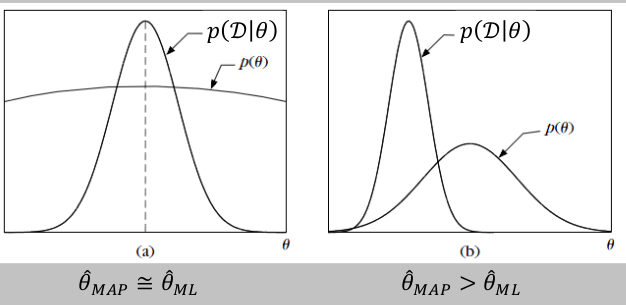
\includegraphics[width=\textwidth]{figs/MLEvsMAP.png}

\subsection*{مثال پرتاب سکه}
دوباره به این مثال برمیگردیم. همانطور که در بخش قبل داشتیم تابع 
\lr{likelihood}
برابر است با 
\[p(D|\theta) = \prod_{i=1}^{N} \theta^{x^{(i)}} (1 - \theta)^{(1 - x^{(i)})}\]
و فرض میکنیم که توزیع 
\lr{prior}
مان نیز از نوع توزیع بتا است.
\[p(\theta) = Beta(\theta|\alpha_1, \alpha_0) = \theta^{\alpha_1 - 1}(1 - \theta)^{\alpha_0 -1}\]
بدین ترتیب برای توزیع 
\lr{posterior}
داریم.
\[= \theta^{m + \alpha_1 - 1}(1 - \theta)^{N - m + \alpha_0 - 1} \xrightarrow[]{} p(\theta|D) = Beta(\theta|\alpha_1^{'}, \alpha_0^{'})\]
و 
\[
\alpha_1' = \alpha_1 + m\]
\[\alpha_0' = \alpha_0 + N - m
\]
\end{document}
